\subsection{Убираем специфические частоты}

\def\num{9}
\def\a{3}
\def\from{-2}
\def\to{4}
\def\b{0.5}
\def\c{0.8}
\def\d{8}
\def\T{10}
\def\imageclip{15}

\subsubsection{Рассматриваемая функция} 

Рассмотрим функцию $g(t)$ при параметрах $a=$~\a, $t1 =$~ \from, $t_2 =$~\to ~(см. рисунок~\ref{fig:wave_function_\num}) 
и ее \textit{зашумленную} версию $u(t)$ с параметрами $b =$~\b, $c =$~\c, $d =$~\d ~(см. рисунок~\ref{fig:noised_wave_function_\num}).
на промежутке $[-T/2,~T/2]$ с $T =$~\T.

\FloatBarrier
\subsubsection{Графики рассматриваемой и зашумленной функции}
\begin{figure}[ht!]
    \centering
    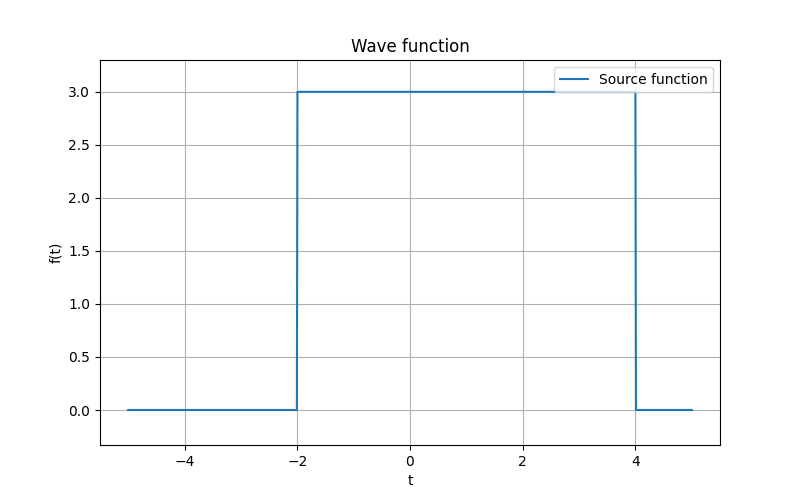
\includegraphics[width=\textwidth]{../results/\num/wave_function.png}
    \caption{Функция $g(t)$ с параметрами $a = \a$, $t_1 = \from$, $t_2 = \to$}
    \label{fig:wave_function_\num}
\end{figure}

\begin{figure}[ht!]
    \centering
    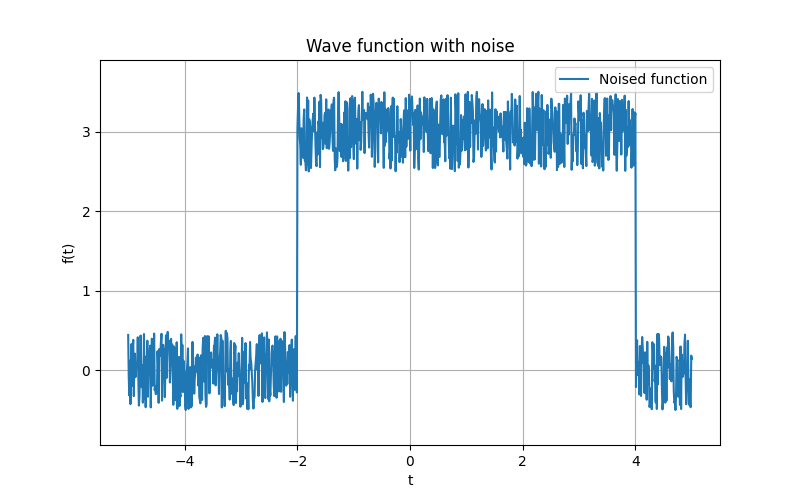
\includegraphics[width=\textwidth]{../results/\num/noised_wave_function.png}
    \caption{Функция $u(t)$ с параметрами $b = \b$, $c = \c$, $d = \d$}
    \label{fig:noised_wave_function_\num}
\end{figure}

Теперь в функции присутствуют обе компоненты шумов -- случайная и гармоническая. Для начала, попробуем избавиться от случайной компоненты уже известным образом. 

\FloatBarrier
\subsubsection{Нахождение образов исходной и зашумленной функций}
Найдем образы исходной (см. рисунок~\ref{fig:wave_function_image_\num}) 
и зашумленной (см. рисуно~\ref{fig:noised_wave_function_image_\num}) функций с помощью преобразования Фурье. 

\begin{figure}[ht!]
    \centering
    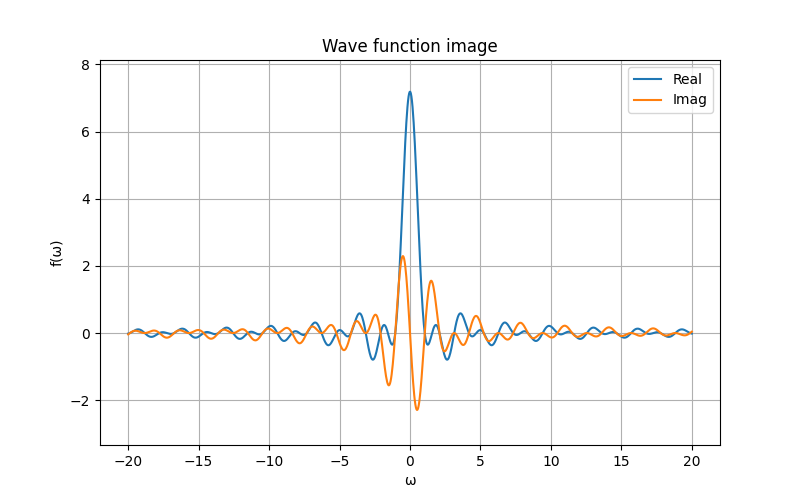
\includegraphics[width=\textwidth]{../results/\num/wave_function_image.png}
    \caption{Образ функция $g(t)$ с параметрами $a = \a$, $t_1 = \from$, $t_2 = \to$}
    \label{fig:wave_function_image_\num}
\end{figure}

\begin{figure}[ht!]
    \centering
    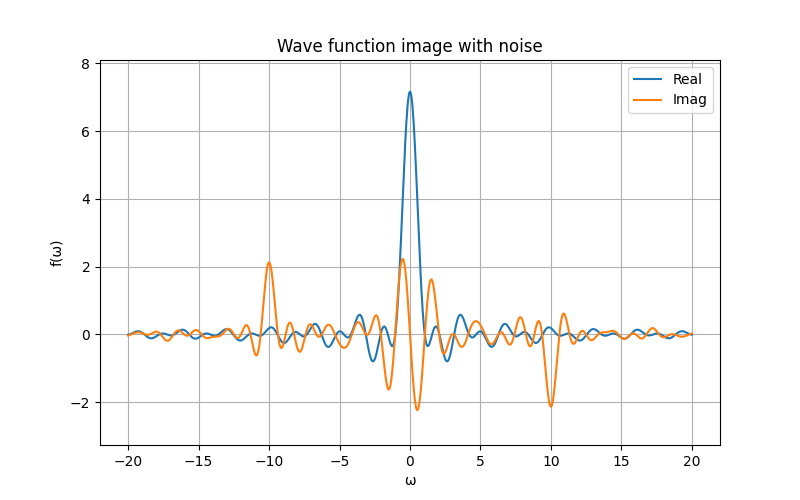
\includegraphics[width=\textwidth]{../results/\num/noised_wave_function_image.png}
    \caption{Образ функция $u(t)$ с параметрами $b = \b$, $c = \c$, $d = \d$}
    \label{fig:noised_wave_function_image_\num}
\end{figure}

\FloatBarrier
\subsubsection{Фильтрация высоких частот}
\textit{Обрежем} образ функции $u(t)$, убрав компоненты, соответствущие высоким частотам (см. рисунок~\ref{fig:noised_wave_function_image_clipped_\num}).

\begin{figure}[ht!]
    \centering
    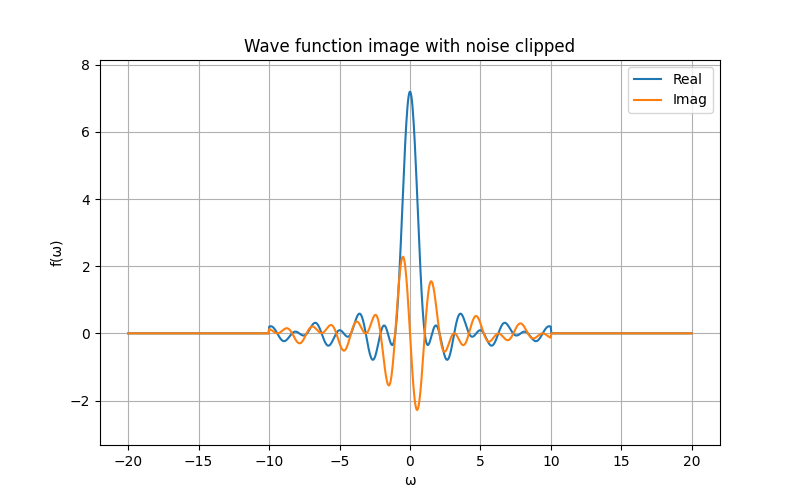
\includegraphics[width=\textwidth]{../results/\num/noised_wave_function_image_clipped.png}
    \caption{Обрезанный образ функция $u(t)$ при $\omega_0=$~\imageclip}
    \label{fig:noised_wave_function_image_clipped_\num}
\end{figure}

Теперь выполним обратное преобразование Фурье (использую обрезанный образ), получив при этом фильтрованную версию функции (см. рисунок~\ref{fig:wave_function_clipped_restored_\num}).

\begin{figure}[ht!]
    \centering
    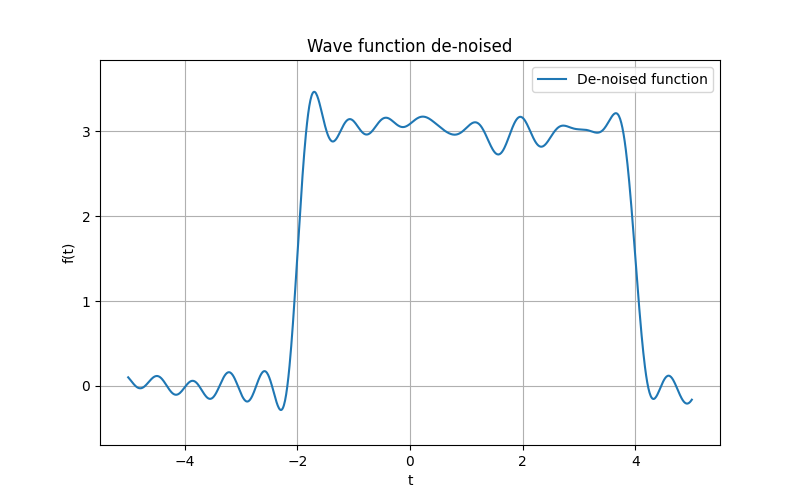
\includegraphics[width=\textwidth]{../results/\num/wave_function_clipped_restored.png}
    \caption{Фильтрованная функция $u(t)$ при $\omega_0=$~\imageclip}
    \label{fig:wave_function_clipped_restored_\num}
\end{figure}

Видим, что соответствущие случайному шуму выбросы исчезли, но в функции все еще присутствует гармоническая составляющая шума. 
Сравнительные графики исходной и фильтрованной функций представлены на рисунке~\ref{fig:wave_function_comparison_\num}. 
\begin{figure}[ht!]
    \centering
    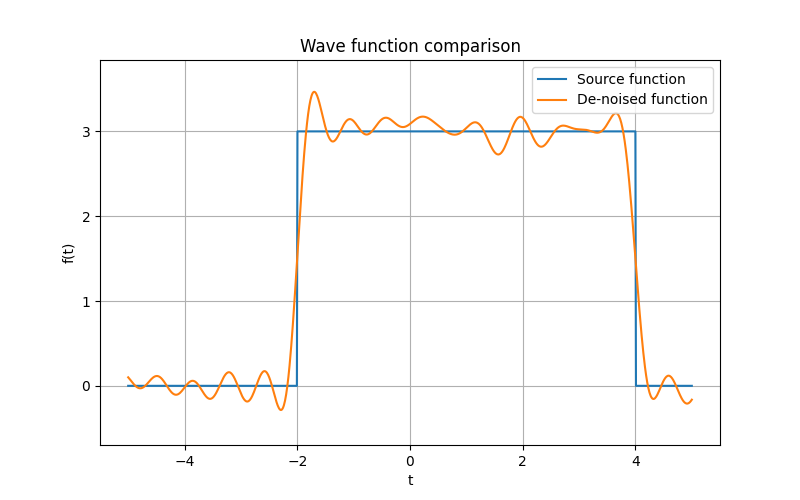
\includegraphics[width=\textwidth]{../results/\num/wave_function_comparison.png}
    \caption{Исходная и фильтрованная функция при $\omega_0=$~\imageclip}
    \label{fig:wave_function_comparison_\num}
\end{figure}

\FloatBarrier
Теперь попробуем избавиться от гармонической составляющей шума. 
Обратим внимание на образ функции $u(t)$ (см. рисунок~\ref{fig:noised_wave_function_image_\num}).
На нем четко видны пики при $\omega = $~\d, что соотносится с тем, что мы положили значение параметра $d$, то есть частоты гармонического шума равным \d.

Для того, чтобы убрать эту компоненту шума обнулим образ функции еще и в небольшой окрестности пиков. В данном случае можно задать \textit{обрезанный} образ 
следующим образом: 
\begin{equation}
    \hat{U}'(\omega) = \begin{cases}
        0, & |\omega| > \omega_0 \\
        0, & \omega \in [\d - \Delta,~\d + \Delta] \\
        0, & \omega \in [-\d - \Delta,~-\d + \Delta] \\
        \hat{U}(\omega), & otherwise
    \end{cases}
\end{equation}
где $\Delta$ -- некоторая малая величина, определяющая ширину окрестности пиков.
Для примера рассмотри случай $\Delta = 0.7$.

\def\num{10}
График полученного образа приведен на рисунке \ref{fig:noised_wave_function_image_clipped_\num}.

\begin{figure}[ht!]
    \centering
    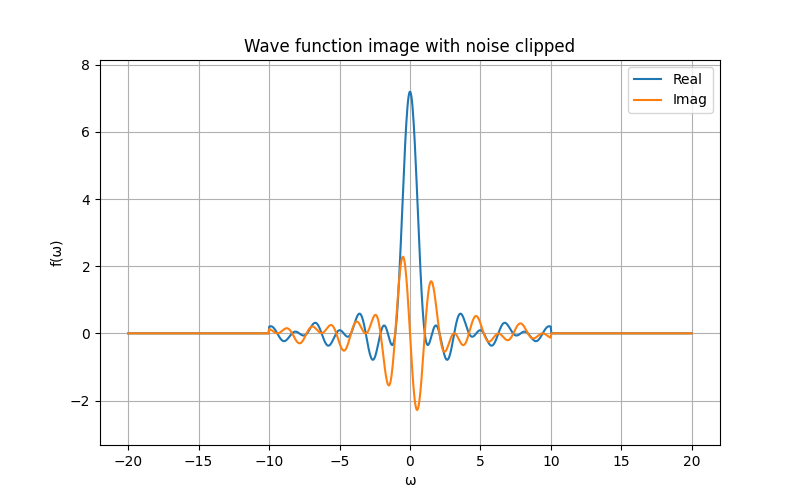
\includegraphics[width=\textwidth]{../results/\num/noised_wave_function_image_clipped.png}
    \caption{Обрезанный образ функция $u(t)$ при $\omega_0=$~\imageclip~и $\Delta = 0.7$, $d = \d$}
    \label{fig:noised_wave_function_image_clipped_\num}
\end{figure}

Теперь выполним обратное преобразование Фурье (используя обрезанный образ), получив при этом фильтрованную версию функции (см. рисунок~\ref{fig:wave_function_clipped_restored_\num}).

\begin{figure}[ht!]
    \centering
    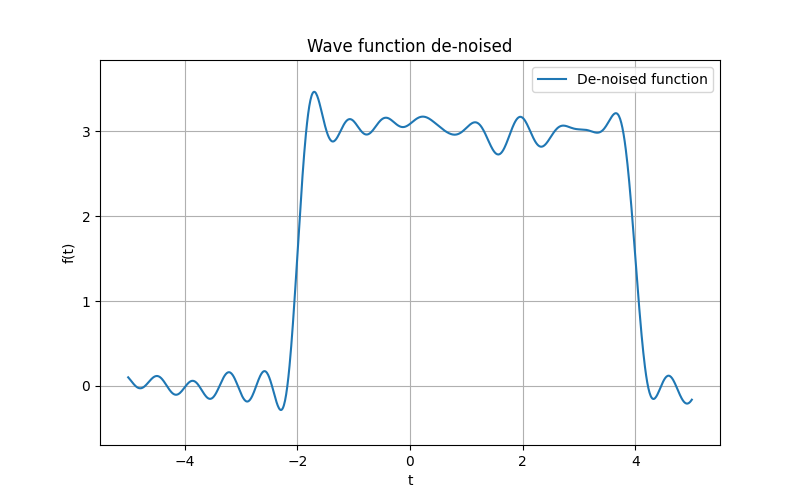
\includegraphics[width=\textwidth]{../results/\num/wave_function_clipped_restored.png}
    \caption{Фильтрованная функция $u(t)$ при $\omega_0=$~\imageclip~и $\Delta = 0.7$, $d = \d$}
    \label{fig:wave_function_clipped_restored_\num}
\end{figure}

Сравнительные графики исходной и фильтрованной функций представлены на рисунке~\ref{fig:wave_function_comparison_\num}. 
\begin{figure}[ht!]
    \centering
    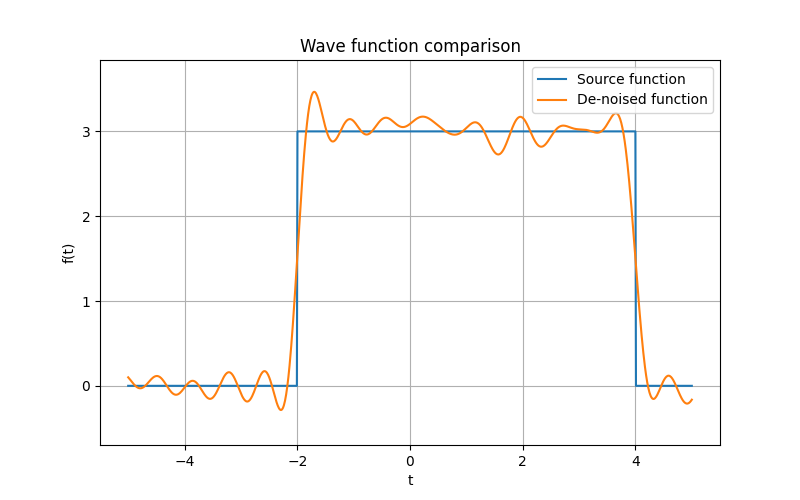
\includegraphics[width=\textwidth]{../results/\num/wave_function_comparison.png}
    \caption{Исходная и фильтрованная функция при $\omega_0=$~\imageclip~и $\Delta = 0.7$, $d = \d$}
    \label{fig:wave_function_comparison_\num}
\end{figure}

Видно, что гармоническую составляющую шума удалось убрать, но при этом исходная функция тоже несколько исказилась. 

\FloatBarrier
\subsubsection{Сравнение модулей образов}
Сравним модули образов исходной и фильтрованной функций (см. рисунок~\ref{fig:wave_function_image_abs_\num}~и~\ref{fig:wave_function_clipped_restored_image_abs_\num}).

\begin{figure}[ht!]
    \centering
    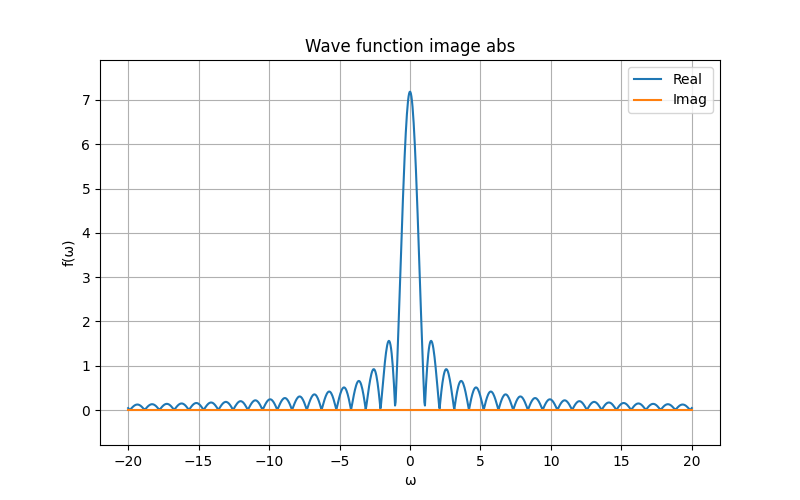
\includegraphics[width=\textwidth]{../results/\num/wave_function_image_abs.png}
    \caption{Модуль образа исходной функции $g(t)$}
    \label{fig:wave_function_image_abs_\num}
\end{figure}

\begin{figure}[ht!]
    \centering
    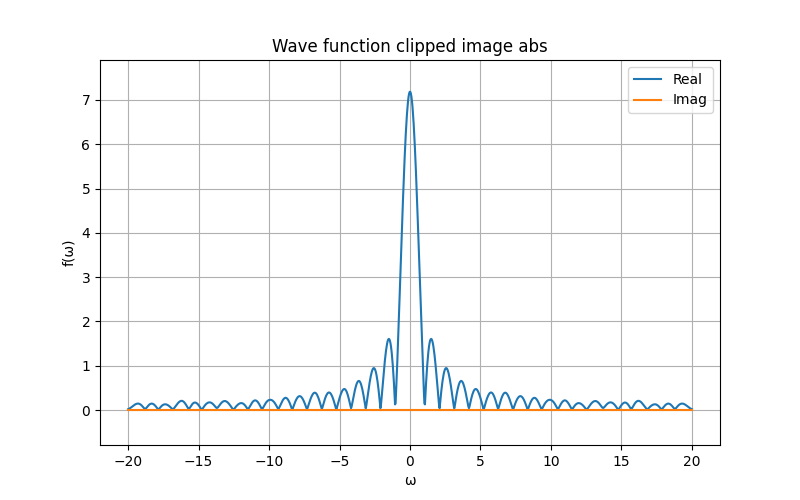
\includegraphics[width=\textwidth]{../results/\num/wave_function_clipped_restored_image_abs.png}
    \caption{Модуль образа фильтрованной функции $u(t)$ при $\omega_0=$~\imageclip}
    \label{fig:wave_function_clipped_restored_image_abs_\num}
\end{figure}

Видим, что практически частоты выше $\omega_0$ обнулились, при этом низкочастотные компоненты остались практически неизменными. 
На графике модуля образа \textit{выбросы}, соответствущие гармоническому шуму не заметы, так как они проявляются только в 
мнимой части образа из-за того, что гармонической составляющей шума соответствует нечетная функция -- синус. 

\FloatBarrier
Таким образом, удалось убрать обе компоненты шума, не сильно изменив при этом вид исходной функции. 

\FloatBarrier
\subsubsection{Только гармонический шум}

\def\num{11}
\def\b{0}
\def\c{1}
\def\d{10}
\def\T{10}

Рассмотрим функцию $g(t)$ при параметрах $a=$~\a, $t1 =$~ \from, $t_2 =$~\to 
и ее \textit{зашумленную} версию $u(t)$ с параметрами $b =$~\b, $c =$~\c, $d =$~\d ~(см. рисунок~\ref{fig:noised_wave_function_\num}).
на промежутке $[-T/2,~T/2]$ с $T =$~\T.
Такой шум имеет только гармоническую составляющую. Такую составляющую можно убрать, обрезав образ функции в окрестности пика, соответствущего нужно частоте. 

\begin{figure}[ht!]
    \centering
    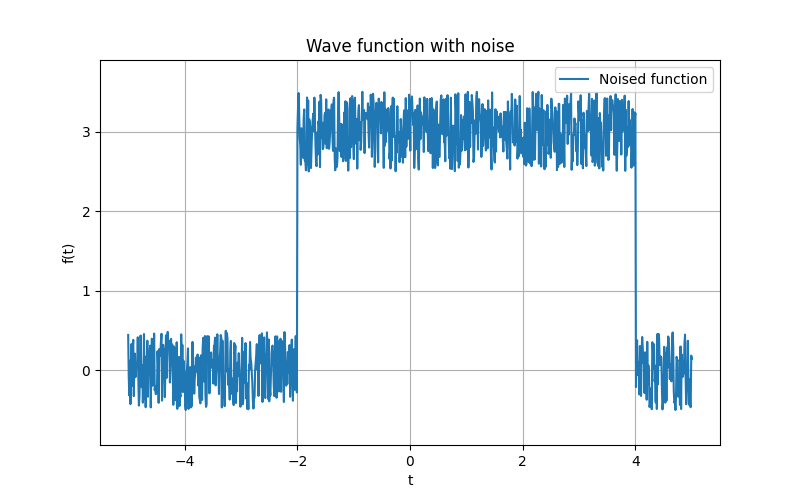
\includegraphics[width=\textwidth]{../results/\num/noised_wave_function.png}
    \caption{Функция $u(t)$ с параметрами $b = \b$, $c = \c$, $d = \d$}
    \label{fig:noised_wave_function_\num}
\end{figure}

\begin{figure}[ht!]
    \centering
    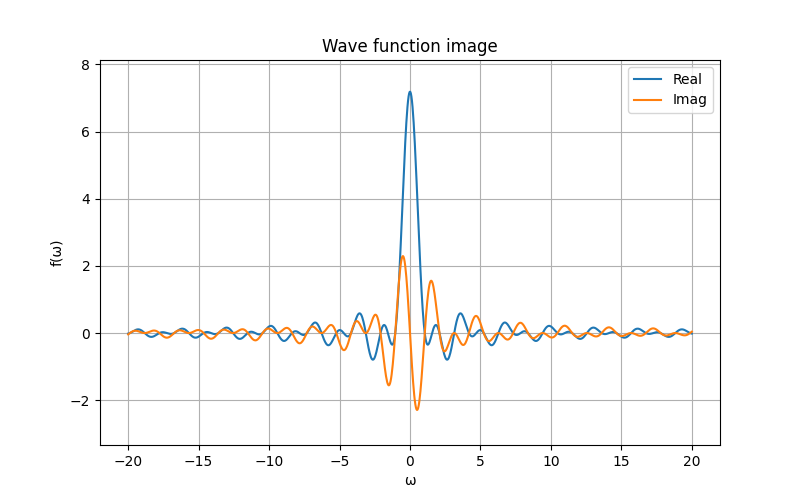
\includegraphics[width=\textwidth]{../results/\num/wave_function_image.png}
    \caption{Образ функция $g(t)$ с параметрами $a = \a$, $t_1 = \from$, $t_2 = \to$}
    \label{fig:wave_function_image_\num}
\end{figure}

\begin{figure}[ht!]
    \centering
    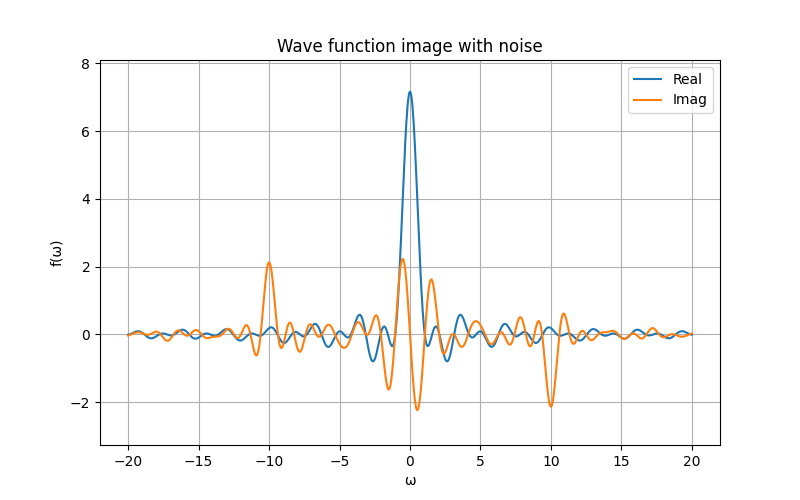
\includegraphics[width=\textwidth]{../results/\num/noised_wave_function_image.png}
    \caption{Образ функция $u(t)$ с параметрами $b = \b$, $c = \c$, $d = \d$}
    \label{fig:noised_wave_function_image_\num}
\end{figure}

\FloatBarrier
На графике образа функции с таким видом шума видно, что пики при $|\omega| = $~\d~(см. рисунок~\ref{fig:noised_wave_function_image_\num})

Обнулим образ в окрестности пика, соответствующего частоте \d. Для примера рассмотри случай $\Delta = 1$.
\begin{figure}[ht!]
    \centering
    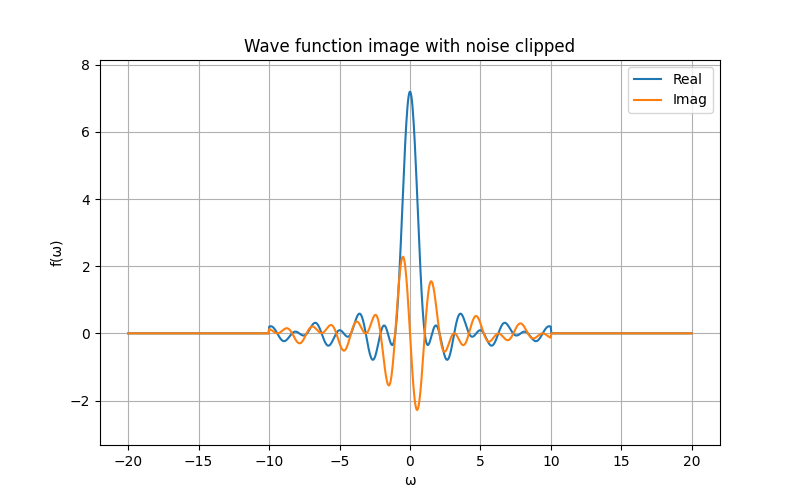
\includegraphics[width=\textwidth]{../results/\num/noised_wave_function_image_clipped.png}
    \caption{Обрезанный образ функция $u(t)$}
    \label{fig:noised_wave_function_image_clipped_\num}
\end{figure}

\begin{figure}[ht!]
    \centering
    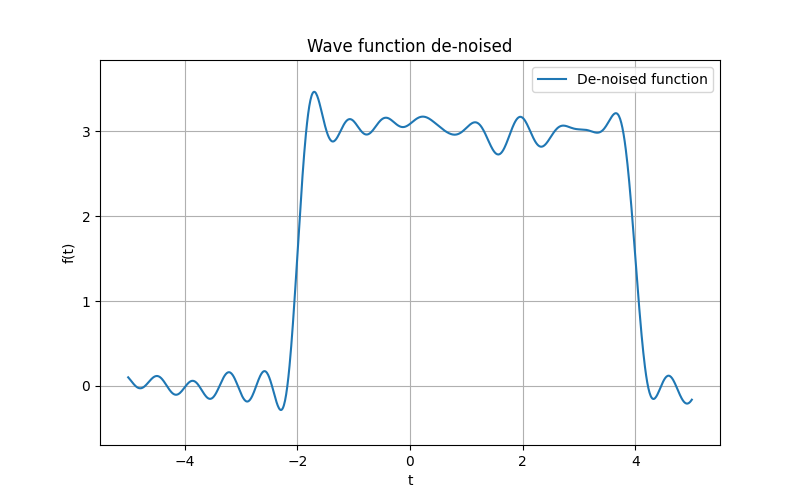
\includegraphics[width=\textwidth]{../results/\num/wave_function_clipped_restored.png}
    \caption{Фильтрованная функция $u(t)$ при $\omega_0=$~\imageclip}
    \label{fig:wave_function_clipped_restored_\num}
\end{figure}

Сравнительные графики исходной и фильтрованной функций представлены на рисунке~\ref{fig:wave_function_comparison_\num}. 
\begin{figure}[ht!]
    \centering
    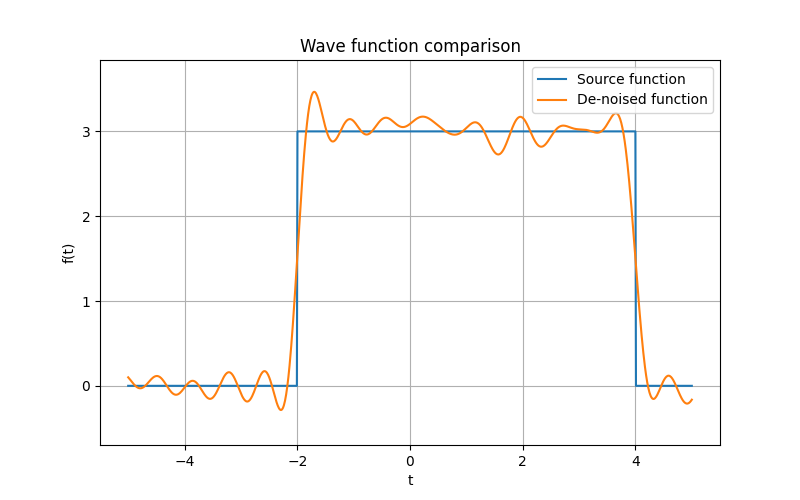
\includegraphics[width=\textwidth]{../results/\num/wave_function_comparison.png}
    \caption{Исходная и фильтрованная функция при $\omega_0=$~\imageclip}
    \label{fig:wave_function_comparison_\num}
\end{figure}

Видно, что гармоническую составляющую шума удалось убрать, но при этом исходная функция тоже несколько исказилась. 

\FloatBarrier
\subsubsection{Исследование влияния параметров b, c, d на фильтрацию}

Из формулы \eqref{eq:noise} понятно, что компонента $b$ отвечает за случайный шум, а $c$ и $d$ -- за гармонический, при этом $c$ -- амплитуда, а $d$ -- частота.

Здесь я приведу только сравнительные графики исходной и фильтрованной функций при различных значениях параметров $b$, $c$, $d$. 

\def\num{12}
\def\b{2}
\def\c{1}
\def\d{10}
\begin{figure}[ht!]
    \centering
    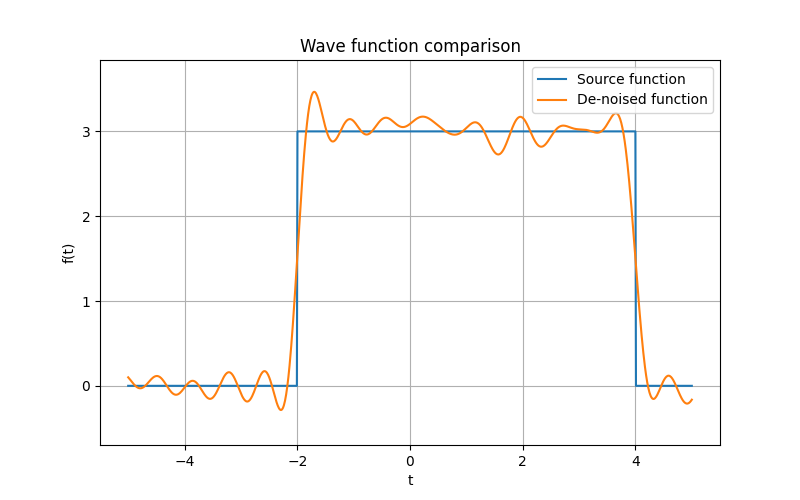
\includegraphics[width=\textwidth]{../results/\num/wave_function_comparison.png}
    \caption{Исходная и фильтрованная функция при $b =$~\b, $c =$~\c, $d =$~\d}
    \label{fig:wave_function_comparison_\num}
\end{figure}

\def\num{13}
\def\b{0.5}
\def\c{3}
\def\d{10}
\begin{figure}[ht!]
    \centering
    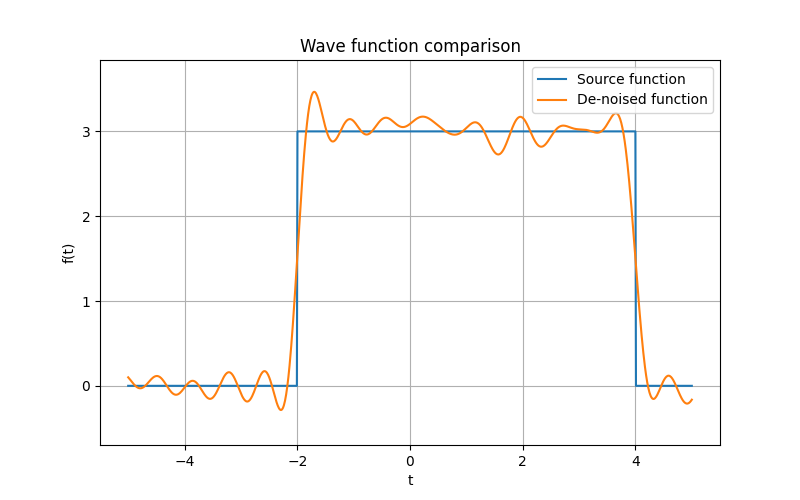
\includegraphics[width=\textwidth]{../results/\num/wave_function_comparison.png}
    \caption{Исходная и фильтрованная функция при $b =$~\b, $c =$~\c, $d =$~\d}
    \label{fig:wave_function_comparison_\num}
\end{figure}

\def\num{14}
\def\b{0.5}
\def\c{1}
\def\d{5}
\begin{figure}[ht!]
    \centering
    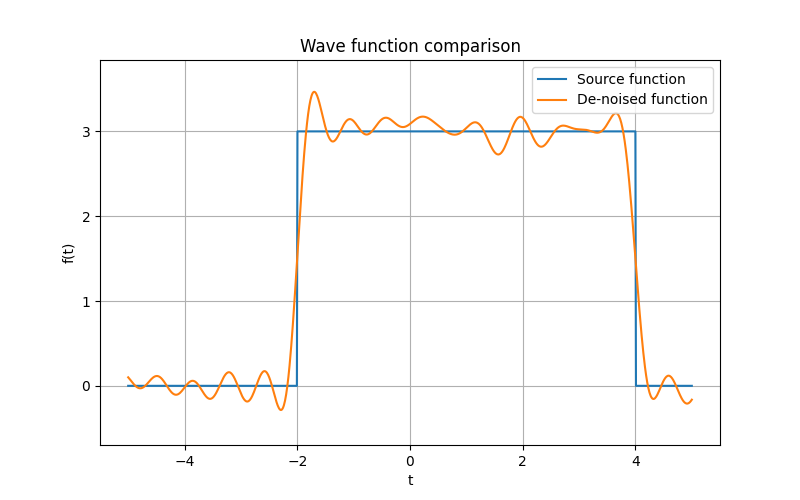
\includegraphics[width=\textwidth]{../results/\num/wave_function_comparison.png}
    \caption{Исходная и фильтрованная функция при $b =$~\b, $c =$~\c, $d =$~\d}
    \label{fig:wave_function_comparison_\num}
\end{figure}

Очевидно, что, чем меньше шума было внесено в функцию, тем лучше будет получаться его убрать. 
Но даже при довольно больших значениях параметров $b$, $c$, $d$ удалось убрать шум, не сильно исказив исходную функцию.